\chapter{Multipath Routing}
\begin{flushright}
 \textit{\textquotedblleft If you want to succeed you should strike out on new paths, \\ 
rather than travel the worn paths of accepted success.\textquotedblright}\\
\textit{-- J. D. Rockefeller}
\end{flushright}
\label{chap:multipath}

\ifpdf
    \graphicspath{{3-MultipathRouting/Chapter2Figs/PNG/}{3-MultipathRouting/Chapter2Figs/PDF/}{3-MultipathRouting/Chapter2Figs/}}
\else
    \graphicspath{{3-MultipathRouting/Chapter2Figs/EPS/}{3-MultipathRouting/Chapter2Figs/}}
\fi

\section{Why Multiple Paths: Some justifications}

Computer networks have grown over the past decades, this growth has lead to a rise in complexity of their topology. While increased complexity is often viewed negatively, it may be a blessing in disguise to networks because it can provide multiple paths towards a destination. If we are able to utilize these alternative paths intelligently, we can expect ta significant increease in network performance.

\ifigure{multipath}{0.5}{A complex network}{fig:ComplexNet}

Figure \ref{fig:ComplexNet} shows a complicated network consisting of multiple paths between a given source-destination pair. For example, consider source A and destination C: we have four possible paths from A to C (A-B-C, A-D-C, A-D-B-C, A,D-E-C). Most protocols nowadays, only consider a single path at any given instant. While such a decision reduces the diffculty in building correct routing tables, it comes with a major drawback: instead of using the entire capacity of the network, one will only use a relatively small fraction (in this case, only a fourth is used).

It has been proven that splitting traffic over multiple paths reduces delay while increasing he efficiency of the network \cite{ParaQueue, Huitema}. If all packets of a given communication can be assigned to one path, then we will obtain higher network throughput as several communication can occur simultaneously and lower delays in both absolute terms and delay variations. Moreover, using multiple paths solves another problem which is encountered in single paths routing: link failure. If a link fails in a multipath scenario, then the traffic can simply be rerouted via an alternative path while a recalculation occurs or the failed path is re-established contrasting with single path routing where the routing tables must be recalculated and all traffic is lost in the meantime. 

%possibly talk about congestion???

On the other hand, splitting traffic over multiple paths comes with its own problems. First, it is possible that packets on different paths encounter different path MTU (Maximum Transmission Unit) and therefore would require a router to break up packets according to the path they take, thereby negating the advantage of an advertised MTU. Second, debugging tools, such as traceroute or ping,  are made inaccurate or even incorrect due to the use multipaths. Finally, a much more serious problem, is the phenomenon of variable delays encountered by packets on different paths which cause them to arrive out of order. In many TCP (Transmission Control Protocol \cite{TCP}) implementations, out of order packets cause retransmissions which drastically reduce the performance of a network. A solution to this problem is suggested in Section \ref{sect:eqcostmulti}.

Before we continue, we must introduce the concept of \textit{flow}, which in this document is similar to the definition of a microflow in \cite{RFC2474}. 

%\newtheorem{definition}{Definition}
\begin{definition}
 A \emph{flow} is a sequence of packets which is identified by its characteristics, such as source and destination address, source and  destination port. Where characteristics could for example be same header values.
\end{definition}

There are two features which are desirable for multipath protocols:
\begin{itemize}
 \item \textbf{Minimal Disruptions} - Since multipath protocol route traffic on many paths, the probability of one path failing or removed for an arbitrary reason is much greater than in the case of single path. It is therefore desirable to minimize the number of flows affected by a link removal.
 \item \textbf{Fast Computation} - The overhead required to compute the next hop to forward a packet or flow should be small when compared with single path protocols.
\end{itemize}


Multipath routing, essentially, asks the question of how to best split network traffic on a set of paths given some cost function. This is known as a flow maximization problem and is a very difficult problem to solve. Moreover, we are not looking for a centralized solution, nor a distributed solution where routers make their own decisions, but a solution based on a feedback loop where decisions are influenced by the evolving network conditions. The centralized solution is NP-Complete, but if we retain some network paths we can solve the problem in a bounded time by assigning a price to each link of the network. The price is the first derivative of the cost function evaluated at the offered traffic level. In order to estimate the offered traffic we must first be aware of all the routing decisions taken by all routers, and therefore this makes such algorithms difficult, if not impossible, to implement in a real network. Moreover, such approaches will inevitably suffer from scalability problems and therefore convergence problems. These problems make up a very active field of research.    


\section{Multipath Routing Schemes}

As it has been shown in the previous section, single path algorithms, such as OSPF, RIP, EIGRP \cite{RIP,OSPF,EIGRP}, make inefficient use of the overall network bandwidth. In this section we present some research multiple paths algorithms whose evolution is shown in Figure \ref{fig:multipathevo}. 

\ifigure{multipathevo}{0.5}{The Evolution of multipath algorithms}{fig:multipathevo}

\subsection{Proposed Extensions to Single Path routing}

Multiple Path Algorithm (MPA) \cite{MPA} is an extension that could be added to OSPF \cite{OSPF}. MPA constructs a subset of paths in a given network which satisfy a condition for loop freeness. This algorithm introduces the notion of a \textit{viable next hop}, where initially the shortest paths are computed. A router then computes the difference between its neighbor's path length to the destination and the distance to get to its neighbor, if this distance is \textbf{less than} the distance from the router to the destination then the path is considered viable. More formally, for every neighbor N of router R the test in Equation \ref{eq:viableroute} is performed:

\begin{equation}
  D_N(R,X) - d(R,N) < D(R,X)
 \label{eq:viableroute}
\end{equation}

Where,
\begin{itemize}
 \item $D_N(R,X)$ is the distance from neighbor N to destination X
 \item $c(R,N)$ is the cost of the link between R and N
 \item $D(R,X)$ is the distance from R to X.
\end{itemize}

\ifigure{MPA}{0.7}{An example of MPA.}{fig:MPA}

If this test is successful then the neighbor is considered a viable next hop. As shown in Figure \ref{fig:MPA}, the path R-N-X is not the shortest path because its total length is 11 whereas the direct path R-X has a length of 10. According to the viability test in Equation \ref{eq:viableroute}, the path R-N-X can be used as an alternative and it does not create any loops.

The problem with classic routing algorithms is their inability to re-route traffic when one of the paths becomes congested or fails. In 1990, Wang proposed the idea of adding emergency exits for traffic when faced with congestion. Shortest Path First with Emergency Exits (SPF-EE) \cite{SPFEE} behaves like a classic algorithm under light traffic conditions, but provides alternate routes when congestion or failures occur rather than updating the routes which is an expensive process. 

Figure \ref{fig:SPFEE} illustrates the idea behind SPF-EE. If the network load is low then a source router S forwards packets along its shortest path to the destination D (denoted SP in Figure \ref{fig:SPFEE}). In the event of some failure, two cases have to be distinguished:

\begin{enumerate}
 \item The alternative path's next hop is downstream from the source router S.
 \item All the neighbors to S, other than the shortest path next hop, are upstream.
\end{enumerate}

\begin{figure}
  \centering
  \subfloat[]{\label{fig:SPFEEa}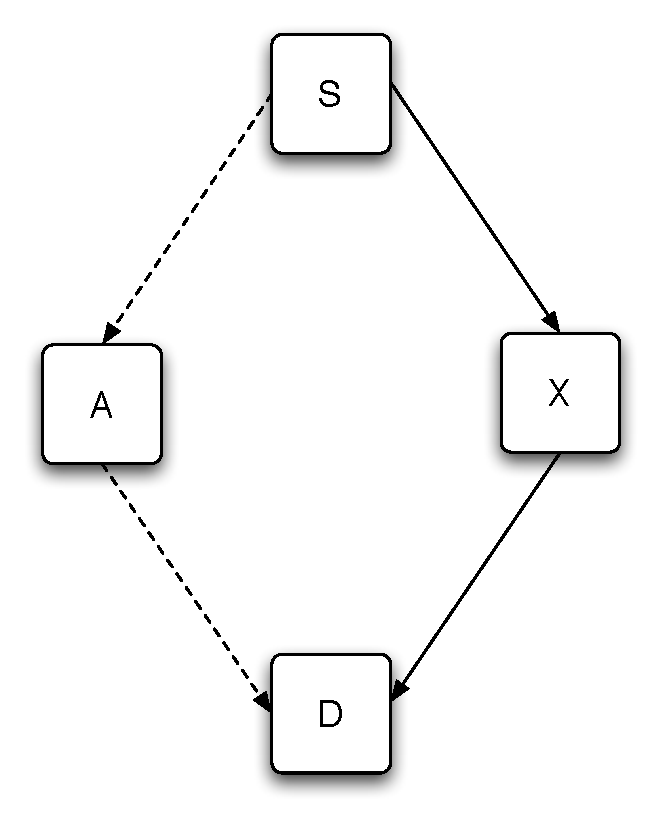
\includegraphics[width=0.3\textwidth]{SPFEEa}}
  \subfloat{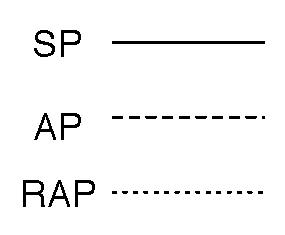
\includegraphics[width=0.2\textwidth]{SPFEELegend}}                 
  \setcounter{subfigure}{1}
  \subfloat[]{\label{fig:SPFEEb}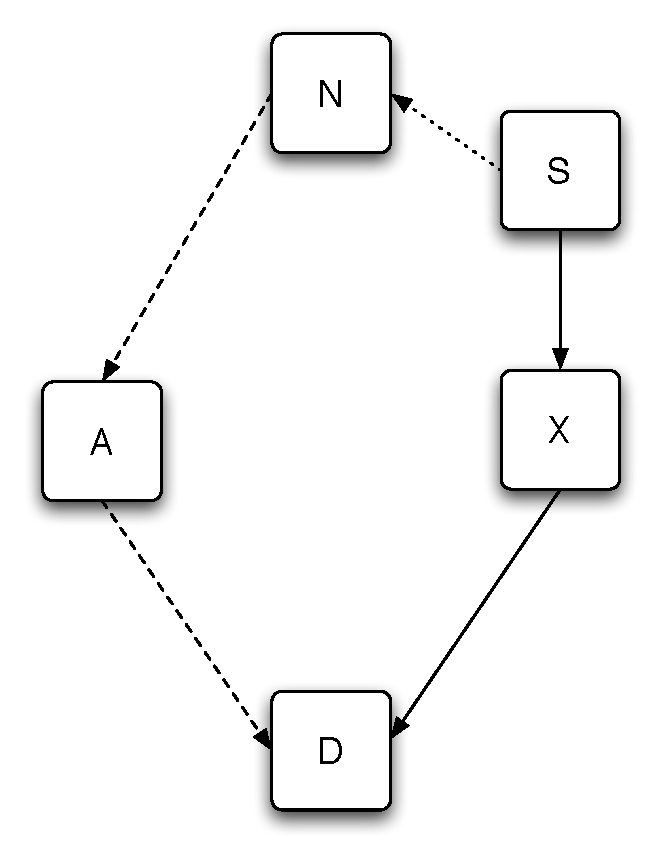
\includegraphics[width=0.3\textwidth]{SPFEEb}}
  \caption{An example of SPF-EE}
  \label{fig:SPFEE}
\end{figure}

%\ifigure{SPFEE}{0.5}{An example of SPF-EE.}{fig:SPFEE}

In the first case, the packet will simply travel from S to the alternative path (denoted by AP in Figure \ref{fig:SPFEE}) next hop (A) and then follow the shortest path from A to the destination as shown in Figure \ref{fig:SPFEEa}. The second case is more complicated as there are no downstream possibilities (assuming that all routing table updates have taken place, and therefore S knows that its shortest path is down) shown in Figure \ref{fig:SPFEEb}. Router S therefore sends a control packet to all its neighbors asking if they have an alternative path to the destination. If a neighbor router N finds a path then it sends the control packet back to S who then establishes a reverse alternative path (RAP), otherwise the neighbor propagates the request to its neighbor routers excluding S. 

The use of a control packet in SPF-EE is problematic because it increases the packet delay significantly while an alternative is found. Moreover, if the source router has no other neighbors other than the shortest path, the algorithm simply fails. A better solution would be to precompute the alternative path set in order to minimize the delay in the event of a failure.

SPF-EE only re-routes traffic in the event of an overload or a failure, another approach would be to take advantage of the path redundancy continuously. Adaptive MultiPath (AMP) \cite{AMP} does precisely that. AMP is based on providing routers with local network status information by exchanging so-called \textit{backpressure messages} (BM). Thus, enabling routers to adapt continuously to the changing network loads.

When AMP detects congestion on a link, it attempts to shift traffic away from this link. In order to achieve this, a router R connected to the congested link sends to its neighboring routers a BM indicating their contribution to the congested link. The neighboring router which receives this BM then notifies its neighbors of their contribution and so on. The routers then attempt to forward the congestion-inducing traffic onto other routes. Figure \ref{fig:AMP} illustrates the dispersion of the BMs when congestion originates from the Y routers.

\ifigure{AMP}{0.5}{An example of AMP.}{fig:AMP}

The issue with such an approach is that while router R knows how much traffic is sent to the individual Y routers, it generates a single value which is then sent back to router X in the form of a BM. Thereby the information which router X is interested in, namely its contribution to the congestion on a given path, is lost. By analyzing the structure of the BMs, we notice that every router needs to maintain a counter for each flow and store a reference of the flows origin because each router needs to compute a BM containing a value which is composed of the contributions of each individual flow, this clearly poses a scalability problem. The derivation of the BMs can be found in Section \ref{sect:AMPCALC}. 

\subsection{Multipath Routing Algorithms}

In 1998, Zauman introduced a new algorithm for the computation of multiple loop free paths from a source to a destination called Diffusing Algorithm for Shortest Multipath (DASM) \cite{DASM}. DASM is based on a generalization of the Diffusing Computations introduced by Dijkstra \cite{DijkstraTerm} and therefore it is also a generalization of DUAL \cite{DUAL} described in Section \ref{sect:DUAL}. DUAL only maintains a single next hop for any destination whereas DASM maintains a set of possible next hops. DASM introduces the concept of the \textit{Shortest Multipath}, which is an extension of DUAL's loop free routing along shortest paths. In DASM, the Shortest Multipath is guaranteed to be acyclic at the end of the diffusing computation.

%\newtheorem{def:shotestmulti}{Definiton}
\begin{definition}
  A \emph{shortest multipath} is defined by the directed acyclic graph obtained by the entries of the routing tables at each router in all paths from a source to a destination.
\end{definition}

\ifigure{DASM}{0.5}{An example of Shortest Multipath constructed with DASM.}{fig:DASM}

In order to ensure loop freeness, DASM constructs the Shortest Multipath graph by forcing routers to select next hops whose distance to the destination is less than their own. Figure \ref{fig:DASM}, illustrates the concept of Shortest Multipaths which contains the shortest path along with longer paths. It should be noted that each router computes the possible paths to the destination, therefore the shortest and longer paths at each router represent the shortest path and longer as computed from the current router.

A subsequent extension of DASM is presented in 2001 by Vutukury which provides loop freeness at every instant. Multipath Distance Vector Algorithm (MDVA) \cite{MDVA} is based on EDVA \cite{EDVA} algorithm presented in Section \ref{sect:DUAL}. To provide loop freeness at every instant MDVA makes sure that at every instant during a diffusing computation, a node who reports a distance via a next-hop K must keep K as its next hop at least until the end of the computation. Simply put, by using the loop free conditions enunciated by EDVA and the method to build multiple paths in DASM coupled with the invariance of reported distances during a computation, MDVA is capable of computing loop free multipaths at every instant.

 In link state algorithms, Vutukury proposed MPDA \cite{MPDA} which provides multiple paths of unequal costs to every destination which are loop free at every instant. The idea is to first compute multiple loop free paths using the same method as Near-OPT \cite{NearOPT}, but then use heuristics built on Gallager's Theorem \cite{Gallager-mindelay} to allocate flows to the computed paths and thereby approximating the optimal result presented in Near-OPT. MPDA sends updates to its neighbors and awaits their acknowledgement before sending another update, contrasting with previous algorithms who used diffusing computations which span the entire network, MPDA only sends out information to its neighbors and therefore its synchronization only spans a single hop.

%(see Section \ref{sect:GallagerAlgo})

Along the same lines as MPDA, Vutukury proposed MPATH \cite{MPATH1, MPATH2} which is a distance vector algorithm providing multiple loop free paths using only neighbor information. MPATH exchanges distances to destinations along with the predecessor to the destination, thereby allowing it to compute multipaths using only predecessor information. Similarly to MPDA, MPATH synchronizes only with its neighbors and therefore performs single hop synchronization. MPDA and MPATH differ only in the type of information their participating nodes exchange.

%see survey for help.

\section{Multipath Routing in current IP networks}


\subsection{OSPF Extensions}

\subsubsection{Equal Cost Multipath}
\label{sect:eqcostmulti}

OSPF defines a multipath protocol, called Equal Cost Multipath (ECMP) \cite{OSPF}, which only considers alternative paths of equal length to the shortest path, ie. each router maintains the set of possible next hops whose subsequent paths are of equal cost to the shortest solution. ECMP suffers from out of order packet arrival if routing decisions are taken packet per packet. To solve this problem several solutions are proposed by \cite{RFC2991}, which each define flows and then each flow is assigned to an outgoing port.

\begin{enumerate}
 \item \textbf{Modulo-N Hash} - The router performs a modulo-N operation over the hash of the packet headers which identity a flow. This method results in $\frac{N-1}{N}$ flow disruptions upon a link failure.
 \item \textbf{Hash-Threshold} - The router computes a hash of the packet headers used to identify a flow. The output range of the hash function is mapped against the number of possible next hops such that a the value of the computed hash will indicate which next hop to use. This method results in between $\frac{1}{4}$ and $\frac{1}{2}$ of all flows to be disrupted upon a link failure. This method is analyzed in \cite{RFC2992}. The analysis of the disruptions is given in Section \ref{sect:HTE}.
 \item \textbf{Highest Random Weight} - The router computes a key for each next-hop by computing a hash over the fields of a flow, as well the over the address for the next-hop \cite{HRW}. The key which obtains the highest value is selected and therefore so is the next-hop. This method involves N times the number of computation as in Modulo-N hash, but only $\frac{1}{N}$ flows are disrupted upon a link failure.
\end{enumerate}
%Above demonstrations to be given in the appendix?


An alternative approach is proposed by Vutukury \cite{TraffEngMinDelay} in which a key is appended by the source router to each packet belonging to a flow. This key is then used to by each router along the path to the destination to determine the next hop.

\subsubsection{OSPF Weights}

Fortz and Thorup \cite{TrafficEngOSPFWeights} and similarly Wang \cite{WANG01} propose methods to optimize the weights assigned to OSPF links. This centralized approach requires that the weights be precomputed assuming that the required load is known beforehand and that the network is quasi-static. Such assumptions make this solution unrealistic for an arbitrary network.

A typical and naive approach is to include a load metric with the standard distance metric \cite{Huitema}. The combination of these two metrics is then used to compute the shortest paths. This process therefore creates a feedback loop:

\begin{enumerate}
 \item A router receives an update for the different link loads and computes the new shortest paths.
 \item The traffic is now re-routed according to the new shortest paths. This causes the link loads to change and therefore,
 \item A new update message is generated and distributed.
\end{enumerate}

Feedback loops cause routes to oscillate and therefore create out of order packets, which as we have seen cause a significant performance loss. The frequency of the oscillations depends on the duration of the feedback loop. If the loop is slow, the number of oscillations is small but very little is gained over standard OSPF. On the other hand, if the loop is fast and many oscillations occur, we can expect many out of order packets and therefore very poor network performance.

\subsubsection{Optimized Multipath OSPF}

We have seen in the previous subsections techniques which attempt to divide traffic more or less equally among the available path sets. In 1998, Villamizar proposed OSPF Optimized Multipath (OMP) \cite{OMP} which takes into account path loads to distribute traffic efficiently among paths. OMP uses mechanisms already available in OSPF to flood the link information within a subnet \cite{RFC2370}.

Initially the algorithm computes the initial set of possible paths. Then the load on each link is iteratively adjusted according to the load information received from other routers. The following steps describe the process of building the path sets:

\begin{enumerate}
 \item Using a standard shortest path first algorithm the shortest paths to all destinations are computed.
 \item Construct a set of possible alternative paths by inspecting paths from neighbors to destinations and combining them with the links from a given router and these neighbors.
 \item Paths which then have equal costs or are within an acceptable margin of the minimum cost are kept. In order to avoid loops, paths which are longer than the minimal cost will only be kept if their immediate neighbor closer to the destination than the origin router.
\end{enumerate}

Once the possible path sets are established, the router can share load onto the paths. Routers will monitor the links and flood load information when the load changes. Depending on the overall network load, the flooding interval can be as large as 20 minutes if the load is low and 30 seconds otherwise. Every time a router receives new load information it will reexamine its load sharing as explained below:

\begin{enumerate}
 \item Examine all links and determine the critical links, and therefore establish the links with the highest load.
 \item Reduce the load on paths containing critical links.
 \item Increase the load on paths which do not contain critical links.
\end{enumerate}

OMP is still considered an experiment and has not yet been deployed in a production environment. However, it is very promising. In the next section we will discuss other load sharing algorithms which are research experiments.

\subsection{Alternative Methods}

In \cite{BAHK}, the authors introduce a routing scheme which is similar to the idea presented by SPF-EE \cite{SPFEE}. Under light traffic conditions, traffic is routed along the shortest path but as the load increases and congestion becomes significant the algorithm attempts to shift traffic onto less congested paths. To achieve this the algorithm uses two main concepts. The first is the classification of link states to identify more easily congested links. The second, is the computation of acceptable alternative paths which are within an acceptable margin of the shortest path in terms of hop count.

Load sensitive routing has always been hampered by the signaling overheads. Moreover, oscillations occur frequently in the path selection because the routing decisions are taken on out dated information. In \cite{LLIP}, the authors suggest a hybrid approach to solve the efficiency and stability issues, which relies on identifying long lived traffic flows and routing them separately. The algorithm provides load sensitive routing for long lived flows while forwarding short lived flows on preprovisioned static paths. In order to identify long lived flows and ensure stability, routers relate the detection of long lived flows to the timescale of signaling messages. 

A similar approach is suggested in \cite{LEE}, where packets are also grouped into flows to avoid out of order arrivals and long lived flows are also differentiated. Although in \cite{LEE}, the authors suggest that a minimum of flow states should be maintained by the router. This results that a flow is either routed on the primary (shortest) path or on the secondary (alternate) path depending on whether it is long lived or not. Figure \ref{fig:longvsshort} shows this load control mechanism: the flow classifier, identifies long lived flows and stores them in the flow table. Then the packet forwarding module forwards the packets according to the contents of the flow table.

\ifigure{flowclassifier}{0.5}{The flow classifier.}{fig:longvsshort}

A dynamic multipath routing (DPMR) scheme to improve resource utilization of a network carrying
real time traffic by re-routing on going flows through shorter routes is proposed in \cite{DMPR, DEDAS}. These approaches alleviate instantaneous congestion by allowing rerouting of a flow through a longer route. In contrast, in this paper, rerouting of an ongoing flow is allowed only if the new route is more preferable (i.e., shorter) than the current one. DMPR scheme works based on the route length, and is independent of the network congestion. 

\section{Summary}

In this section, we have presented the current state of the art in terms of multipath protocols. We have seen that the current protocols do not use multipath in a dynamic sense. Some protocols only consider paths of equal length, but these paths may not always be available. Other protocols introduce mechanisms for quick failover in case a path breaks. Finally, some protocols are simply not implementable as they will require too many resources. In the next sections, we will introduce models for multipath protocols and describe our congestion-aware protocols.
%Figure evolution from 28 to 32 

%summarize articles 28-32 see survey for help.
  


%\section{MPLS Networks}
%chap 5.

% ------------------------------------------------------------------------

%%% Local Variables: 
%%% mode: latex
%%% TeX-master: "../thesis"
%%% End: 
